% !TEX root = master_thesis.tex
\chapter{Experimental Setup}
As motivated in the previous chapter, it is promising to study the photoproduction of pseudoscalar mesons in order to determine a complete set of polarization observables. This requires a polarized photon beam and/or a polarized target. It is convenient to study photoproduction off a fixed target and investigate the resonances that occur in the process. Incidentally, these resonances can only be accessed via their decay products, such that suitable calorimeters are needed. The CBELSA/TAPS experiment is  located in Bonn  at the ELectron Stretcher Accelerator (ELSA), which can be used to generate a high energy photon beam using the \emph{bremsstrahlung} process, meets all above mentioned requirements. This chapter will elaborate on the already mentioned parts of the experiment that was used to collect the data needed for the determination of the target asymmetry in $\eta'$ photoproduction.

\section{Production of (polarized) high energy photon beam}
First of all, a high energy photon beam has to be produced.
\begin{figure}[htbp]
	\centering
	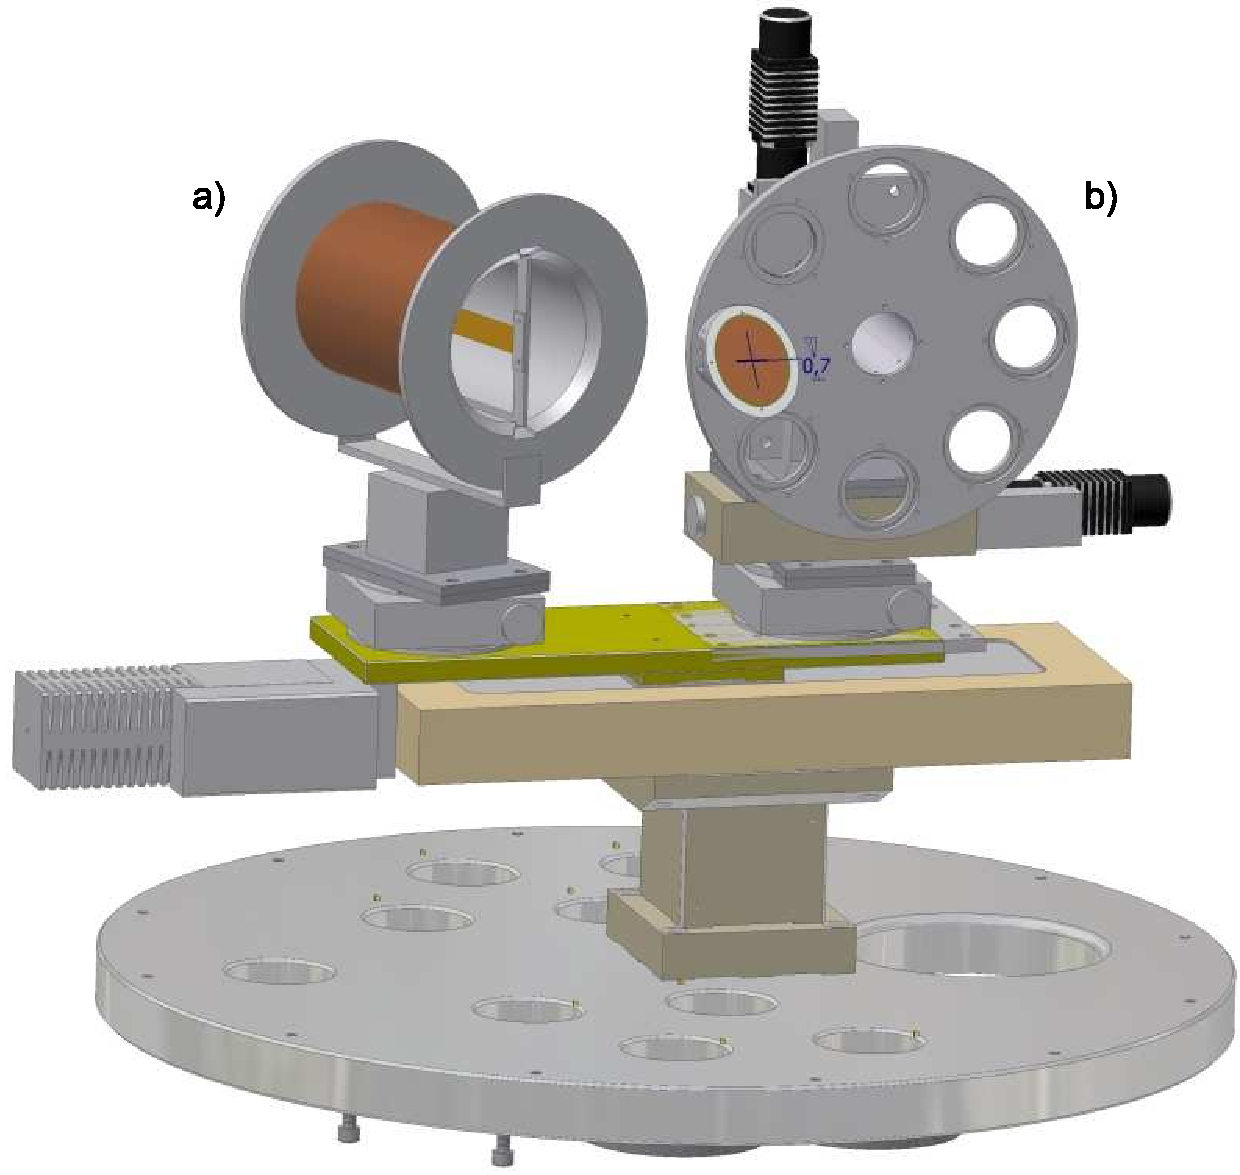
\includegraphics[width=.49\linewidth]{figs/goni-ganz.pdf}
	\caption{\cite{cb}}
\end{figure}
\begin{figure}[htbp]
	\centering
	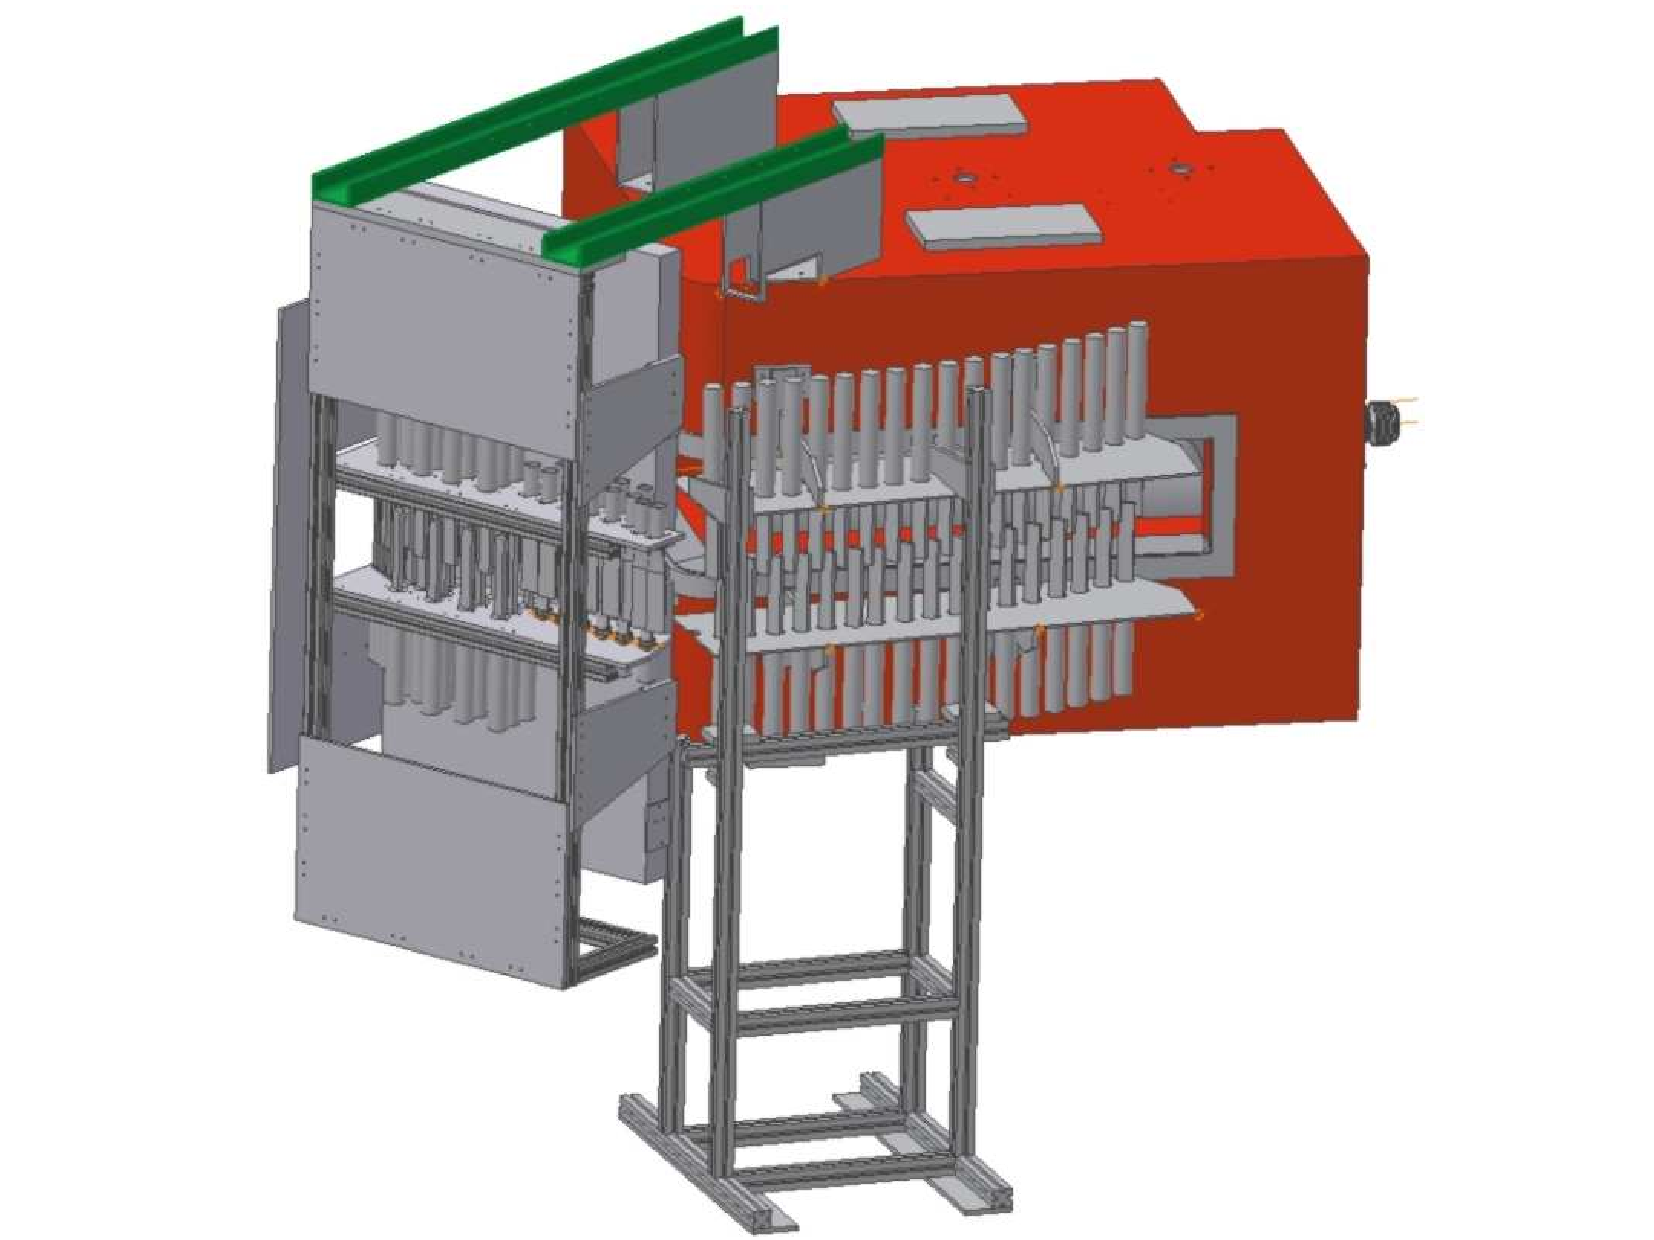
\includegraphics[width=.49\linewidth]{figs/Tagger.pdf}
	\caption{\cite{cb}}
\end{figure}

\section{Beam Target}

\begin{figure}[htbp]
	\centering
	\includegraphics[width=.5\linewidth]{figs/Target.pdf}
	\caption{\cite{cb}}
\end{figure}
\section{Calorimeters}
\begin{figure}[htbp]
	\centering
	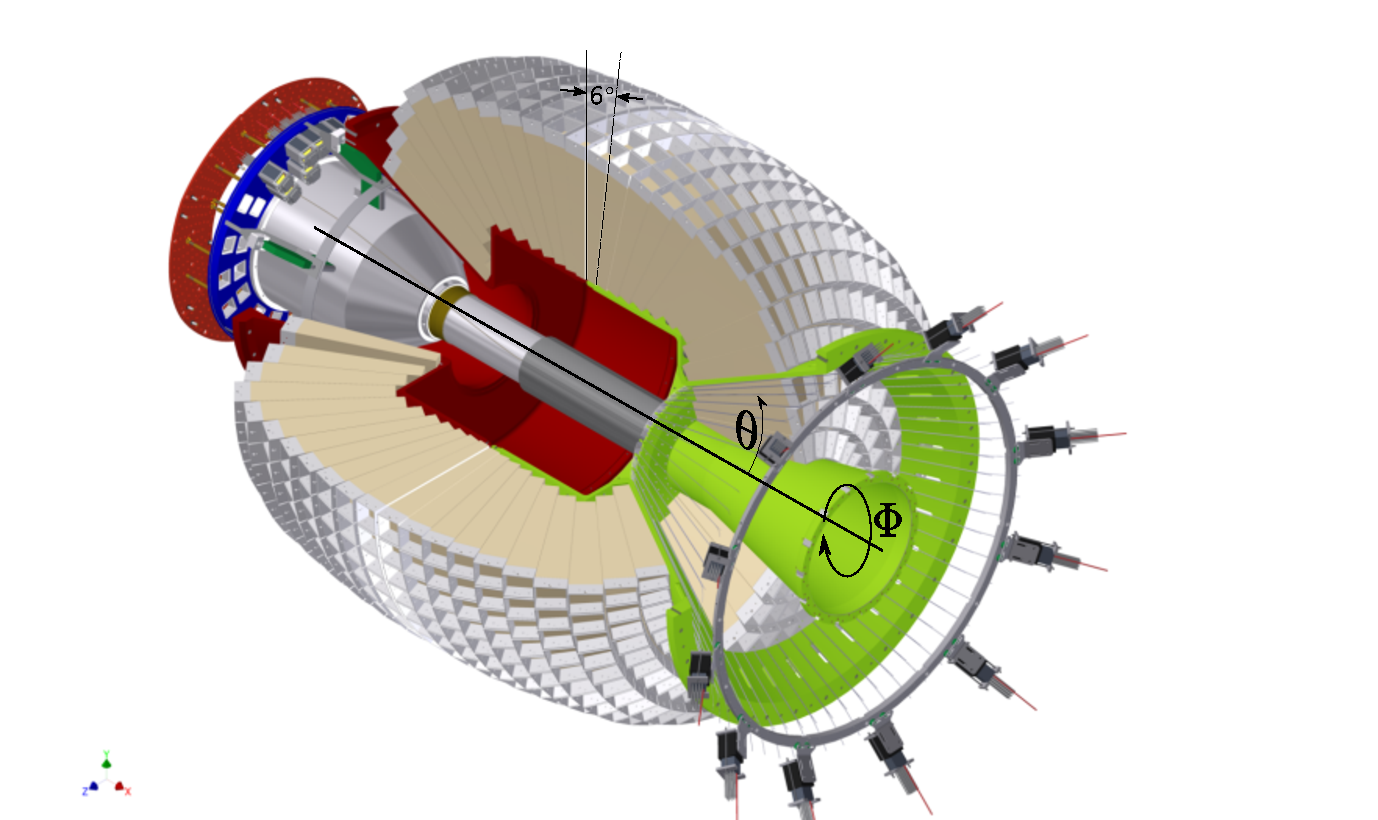
\includegraphics[width=\linewidth]{figs/cb_fp_in.pdf}
	\caption{\textsc{D. Walther} in \cite{urban}}
\end{figure}
\begin{figure}[htbp]
	\centering
	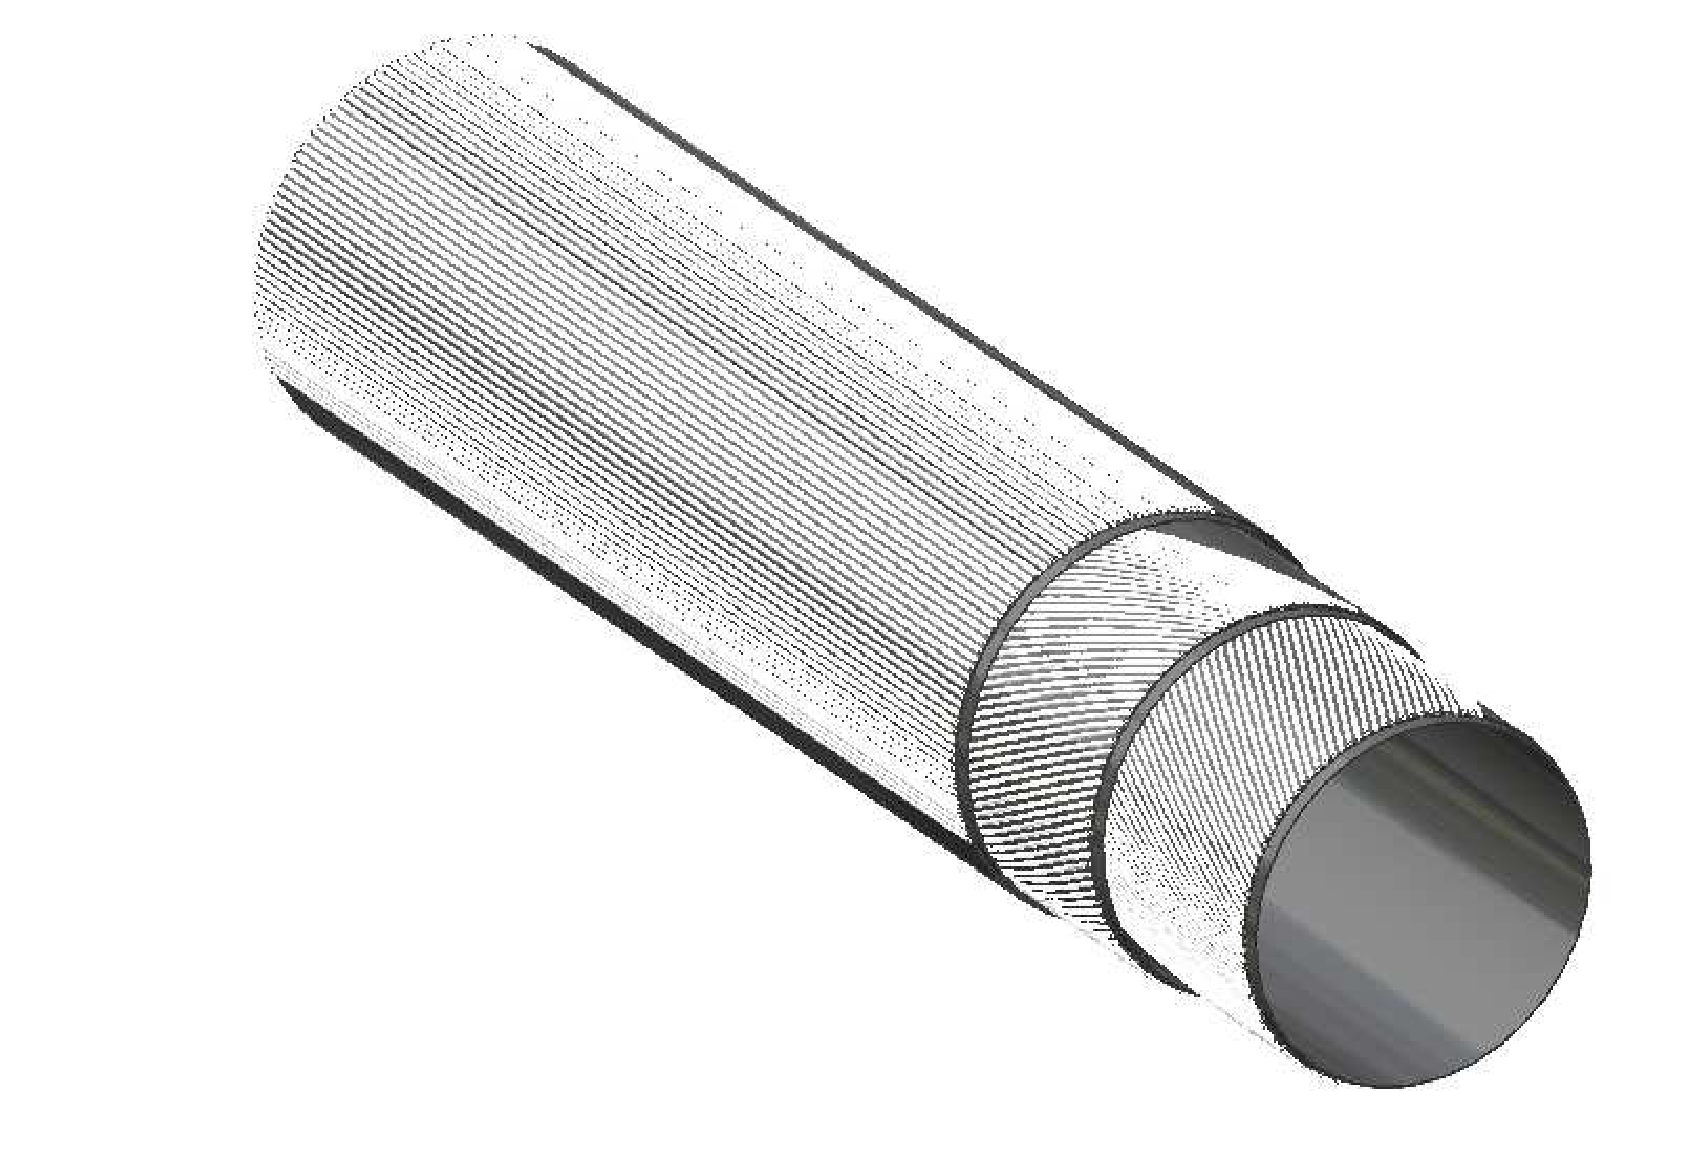
\includegraphics[width=.5\linewidth]{figs/faserorient.pdf}
	\caption{\cite{cb}}
\end{figure}
\begin{figure}[htbp]
	\centering
	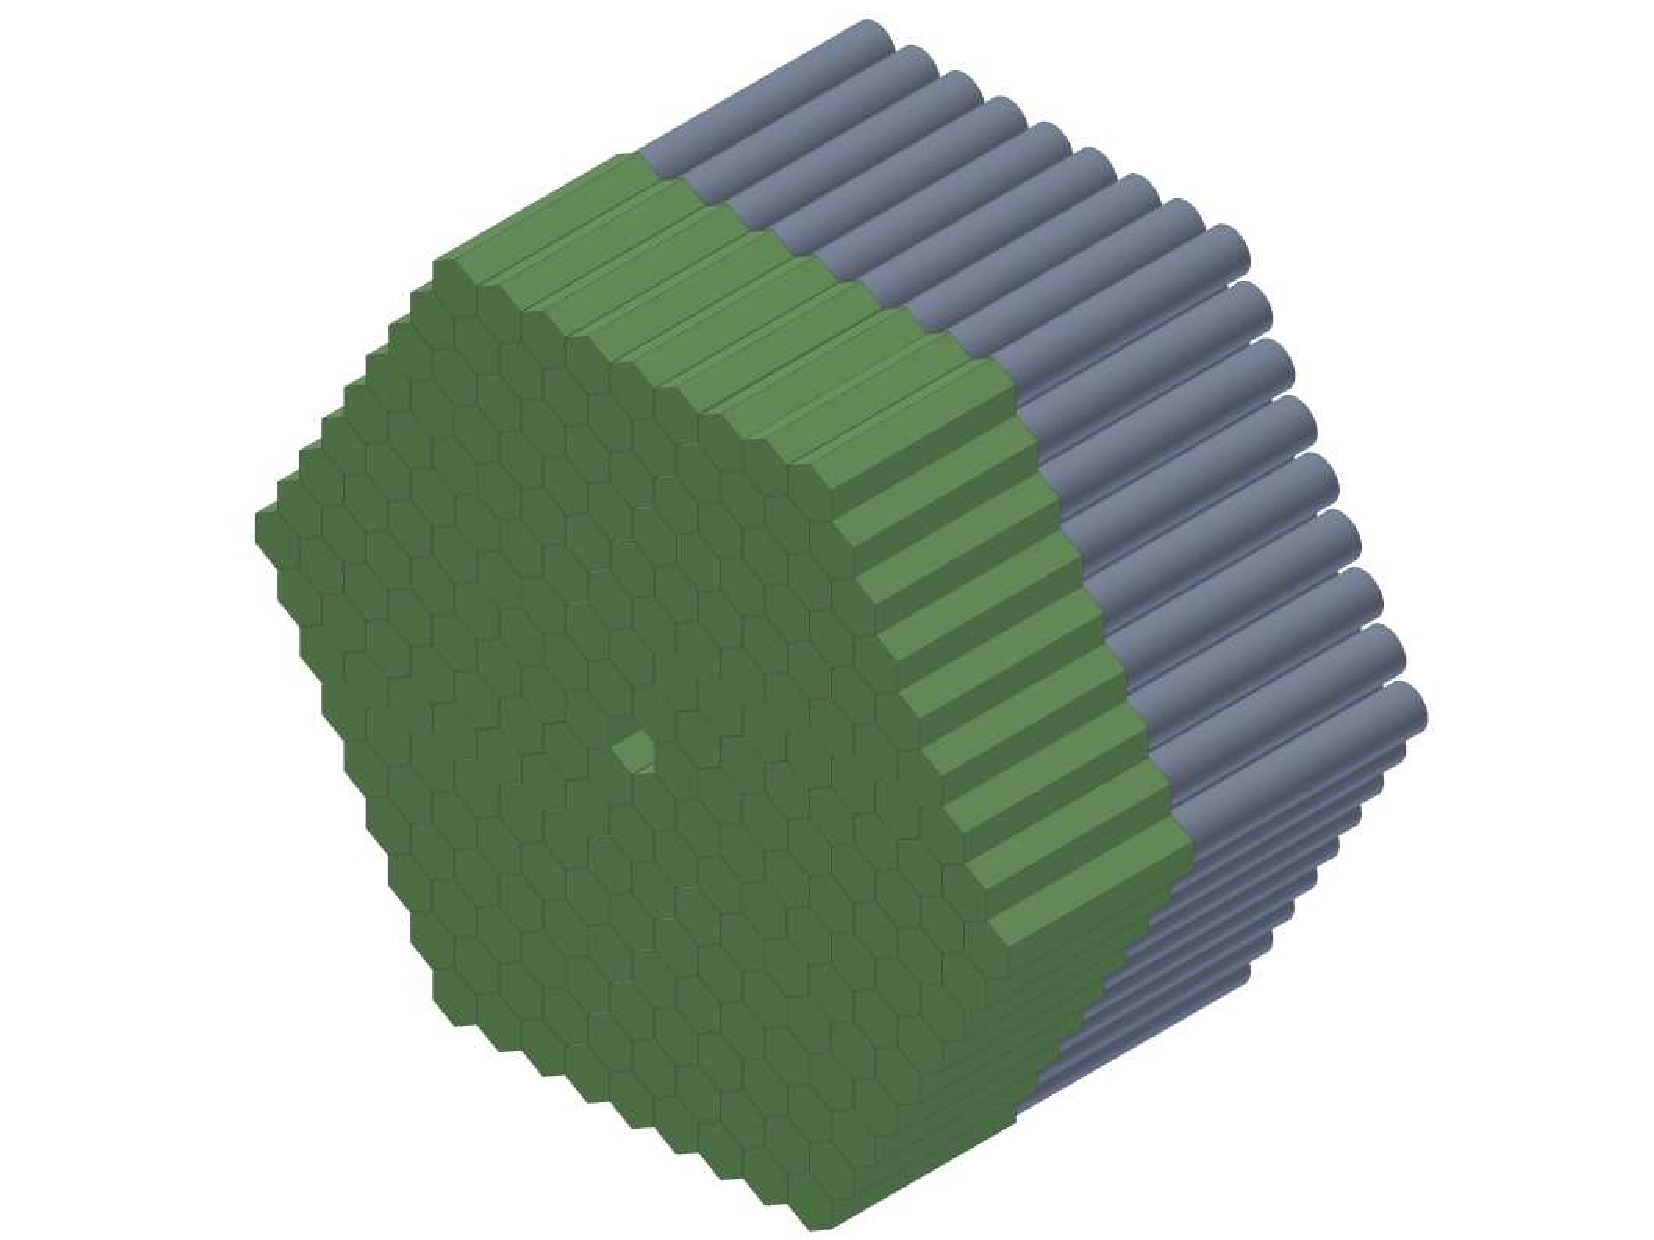
\includegraphics[width=.5\linewidth]{figs/mini-taps.pdf}
	\caption{\cite{cb}}
\end{figure}

\section{Trigger}